\documentclass[a4paper,10pt]{article}
\usepackage[utf8]{inputenc}
\usepackage[nottoc,numbib]{tocbibind} % makes the BibTeX references section appear in the table of contents
\usepackage[inline]{enumitem}
\usepackage{amssymb}
\usepackage{amsfonts}
\usepackage{amsmath}
\usepackage{amsthm}
\usepackage{color}
\usepackage{caption}
\usepackage{subcaption}
\usepackage{graphicx}
\usepackage{mathtools}
\usepackage{mathrsfs}
\usepackage{framed}
% eventually make left/right margins equal
\usepackage[top=0.6in,bottom=0.6in,left=0.1in,right=0.9in]{geometry}
\usepackage{dsfont}



\usepackage[textwidth=0.7in]{todonotes}

\usepackage[hidelinks]{hyperref} %this needs to be loaded last!

% for 3D pictures
\usepackage{tikz}
\usepackage{tikz-3dplot}
\usetikzlibrary{perspective}

%prevent math mode statements from being broken up across lines
\relpenalty=9999
\binoppenalty=9999

%claim environment
\newenvironment{claim}[1]{\par\noindent\underline{Claim:}\space#1}{}

%leftbar
\renewenvironment{leftbar}[1][\hsize]
{%
    \def\FrameCommand
    {%
        {\vrule width 3pt}%
        \hspace{0pt}%must no space.
        \fboxsep=\FrameSep\colorbox{white}%
    }%
    \MakeFramed{\hsize#1\advance\hsize-\width\FrameRestore}%
}
{\endMakeFramed}

% fix footnote spacing
\let\oldfootnote\footnote
\renewcommand{\footnote}{\unskip\oldfootnote}


%numbering and style of theorems
\theoremstyle{plain}
\newtheorem{Theorem}{Theorem}
\newtheorem{Proposition}[Theorem]{Proposition}
\newtheorem{Corollary}[Theorem]{Corollary}
\newtheorem{Lemma}[Theorem]{Lemma}
\newtheorem{Question}[Theorem]{Question}
\newtheorem{Conjecture}[Theorem]{Conjecture}
\newtheorem{Assumption}[Theorem]{Assumption}
\newtheorem{Algorithm}[Theorem]{Algorithm}

\theoremstyle{definition}
\newtheorem{Definition}[Theorem]{Definition}
\newtheorem{Property}[Theorem]{Property}
\newtheorem{Notation}[Theorem]{Notation}
\newtheorem{Condition}[Theorem]{Condition}
\newtheorem{Example}[Theorem]{Example}
\newtheorem{Exercise}[Theorem]{Exercise}
\newtheorem{Introduction}[Theorem]{Introduction}

\theoremstyle{remark}
\newtheorem{Remark}[Theorem]{Remark}
\newtheorem{case}{Case}[Theorem]

% make proofs use filled in black square instead of empty square
\renewcommand{\qedsymbol}{$\blacksquare$}
%\renewcommand\proof{\noindent\textit{\textbf{Proof. }}}
\newcommand{\modo}[3]{#1 \equiv #2 \pmod{#3}}
\newcommand{\nmodo}[3]{#1 \not\equiv #2 \pmod{#3}}
\newcommand{\R}{\mathbb{R}}
\newcommand{\Q}{\mathbb{Q}}
\newcommand{\N}{\mathbb{N}}
\newcommand{\Z}{\mathbb{Z}}
\newcommand{\Zpos}{\mathbb{Z}_{\geq 0}}
\renewcommand{\vec}[1]{\mathbf{#1}}
\newcommand{\dist}{\text{dist}}
\newcommand{\F}{\mathbb{F}}
\newcommand{\C}{\mathbb{C}}
\newcommand{\lin}{\text{lin}}
\newcommand{\cl}{\text{cl}}
\newcommand\norm[1]{\left\lVert#1\right\rVert}
\newcommand{\ONE}{\mathds{1}}
\newcommand{\generatedby}[1]{\left\langle#1\right\rangle}
\newcommand{\id}{\text{id}}
\DeclareMathOperator{\sgn}{sgn}
\newcommand\abs[1]{\left|#1\right|}
\newcommand\Gl{\text{Gl}}
\DeclareMathOperator{\pam}{pam}

\title{Virus Research \\ \large SIP}
\author{Xavier Silva}

\begin{document}

\maketitle

\tableofcontents

% \newpage

\section{Abstract}

Icosahedral viruses have the symmetries of an icosahedron, which involves 2-fold, 3-fold, and 5-fold rotational symmetries.
We can approximate these virus capsids with finite sets of points (called a point array) which we realize in 6D (not just 3D) for the purpose of crystallography: our 6D point arrays naturally fit inside 6D icosahedral lattices. There are \(55\) standard point arrays (called \emph{one-base}) from which we build all the others.
We model virus maturation by 6D linear transformations (transitions) of point arrays that preserve some or all of icosahedral symmetry.
The symmetries we wish to preserve are either full icosahedral, $A_4$ ($3$-fold and $2$-fold), $D_{10}$ ($5$-fold and $2$-fold) or $D_6$ ($3$-fold and $2$-fold) symmetry.
We define full icosahedral symmetry as a group defined by \(\mathcal{I} := \generatedby{a, b | a^2 = b^3 = (ab)^5 = 1}\).
We then notice that \(A_4, D_{10}, \text{ and } D_6\) are maximal subgroups of \(\mathcal{I}\).
To find transitions that preserve one of these symmetry groups, we solve matrix equations of the form \(TB_0 = B_1\) for \(T\), where \(T\) is a \(6\times6\) matrix that depends on either 2, 4, 6, or 8 real variables, depending on which symmetry we are looking at and \(B_0\) and \(B_1\) are representations of the point arrays.
Note that actually finding transitions requires a large amount of computation.
From this we are able to reproduce previously discovered transitions for the Cowpea Chlorotic Mottle Virus that preserve \(D_6\) symmetry, and more importantly create a comprehesive list of what symmetries can be preserved between any possible combination of the \(55\) standard point arrays.

\section{Intro}
Icosahedral viruses have the symmetries of an icosahedron, which involves 2-fold, 3-fold, and 5-fold rotational symmetries.
We can approximate these virus capsids with finite sets of points (called a point array) which we realize in 6D (not just 3D) for the purpose of crystallography: our 6D point arrays naturally fit inside 6D icosahedral lattices. 
There are \(55\) standard point arrays (called \emph{one-base}) from which we build all the others.
We model virus maturation by 6D linear transformations (transitions) of point arrays that preserve some or all of icosahedral symmetry.


% Viruses have a point cloud, we can then lift into 6D dimensions in a non-trivial way.
% These point clouds will then fit into a \emph{lattice}.

Relevant to our work the shape of the icosahedron, a shape with 2-fold, 3-fold, and 5-fold symmetry.
\begin{Definition}[Icosahedral Group]
	The icosahedral group, which we denote by \(\mathcal{I}\), is the 60-element group given by \[\mathcal{I} := \generatedby{a, b | a^2 = b^3 = (ab)^5 = 1}.\]
\end{Definition}
\noindent We realize the icosahedral group as a \( 6 \times 6 \) matrix group.
\begin{Definition}[Generators of the Icosahedral Group]
	A 6D representation of the generators for \(\mathcal{I}\) are as follows:
	\[a = \begin{bmatrix}
		-1 & 0  & 0 & 0 & 0 & 0 \\
		0  & -1 & 0 & 0 & 0 & 0 \\
		0  & 0  & 0 & 0 & 1 & 0 \\
		0  & 0  & 0 & 0 & 0 & 1 \\
		0  & 0  & 1 & 0 & 0 & 0 \\
		0  & 0  & 0 & 1 & 0 & 0
	\end{bmatrix} \quad b = \begin{bmatrix}
		0 & -1 & 0  & 0 & 0 & 0 \\
		0 & 0  & -1 & 0 & 0 & 0 \\
		1 & 0  & 0  & 0 & 0 & 0 \\
		0 & 0  & 0  & 0 & 0 & 1 \\
		0 & 0  & 0  & 1 & 0 & 0 \\
		0 & 0  & 0  & 0 & 1 & 0
	\end{bmatrix}.\]
\end{Definition}

\section{Point Arrays and Lattices}
Icosahedral viruses are characterized by point arrays, which are a set of points in 3 dimensions.
\begin{Definition}[Icosahedral Point Array]
	Let \(\vec{t}, \vec{v}_1, \vec{v}_2, \dots, \vec{v}_n\) be 6 dimensional vectors.
	Then the icosahedral point array generated by these vectors is \[P = \mathcal{I}\vec{v}_1 \cup \mathcal{I}\vec{v}_2 \cup \dots \cup \mathcal{I}\vec{v}_n \cup (\mathcal{I}\vec{v}_1 + \mathcal{I}\vec{t}) \cup (\mathcal{I}\vec{v}_2 + \mathcal{I}\vec{t}) \cup \dots \cup (\mathcal{I}\vec{v}_n + \mathcal{I}\vec{t}).\]
\end{Definition}
Notice that while icosahedral viruses are characterized by 3 dimensional point arrays, \emph{icosahedral point arrays} are 6 dimensional.
This is because we want icosahedral point arrays to fit inside icosahedral lattices, and no such lattices exist in dimensions lower than 6.
\footnote{Because lattices of dimension 5 and lower cannot preserve 5-fold rotational symmetry.}
However, we can project icosahedral point arrays from 6 dimensions into 3 dimensions using the projection matrix given in \cite{indelicatoetal2012}.

There are 55 standard point arrays from which we build all others.
These are called the \emph{one-base} point arrays and take the form \(\mathcal{I}\vec{v} \cup (\mathcal{I}\vec{v} + \mathcal{I}\vec{t})\). This form tells us that only one translation vector and one ``base" vector is needed to create the point array. \cite{keeftwarock2009affine}

\subsection{Constructing Point Arrays}
Constructing a one-base point array involves us finding all vectors in the set \(\mathcal{I}\vec{v} \cup (\mathcal{I}\vec{v} + \mathcal{I}\vec{t})\).
This is shown visually in figure \ref{fig:point_array_construction}.

\begin{figure}[h!]
	\centering
	\begin{subfigure}{0.25\textwidth}
		\centering
		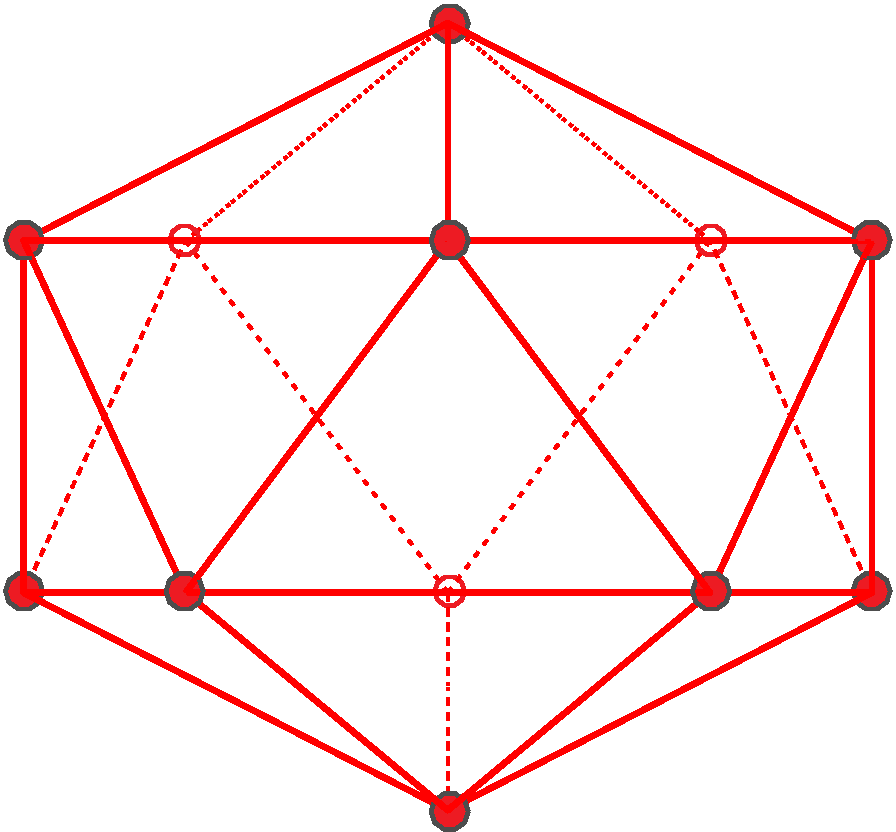
\includegraphics[width=\textwidth]{images/p_arr_construction_1.pdf}
		\caption{Start with icosahedron, created by applying icosahedral symmtry on one vector. Mathematically this is \(\mathcal{I}\vec{v}\).}
	\end{subfigure}
	\hfill
	\begin{subfigure}{0.3\textwidth}
		\centering
		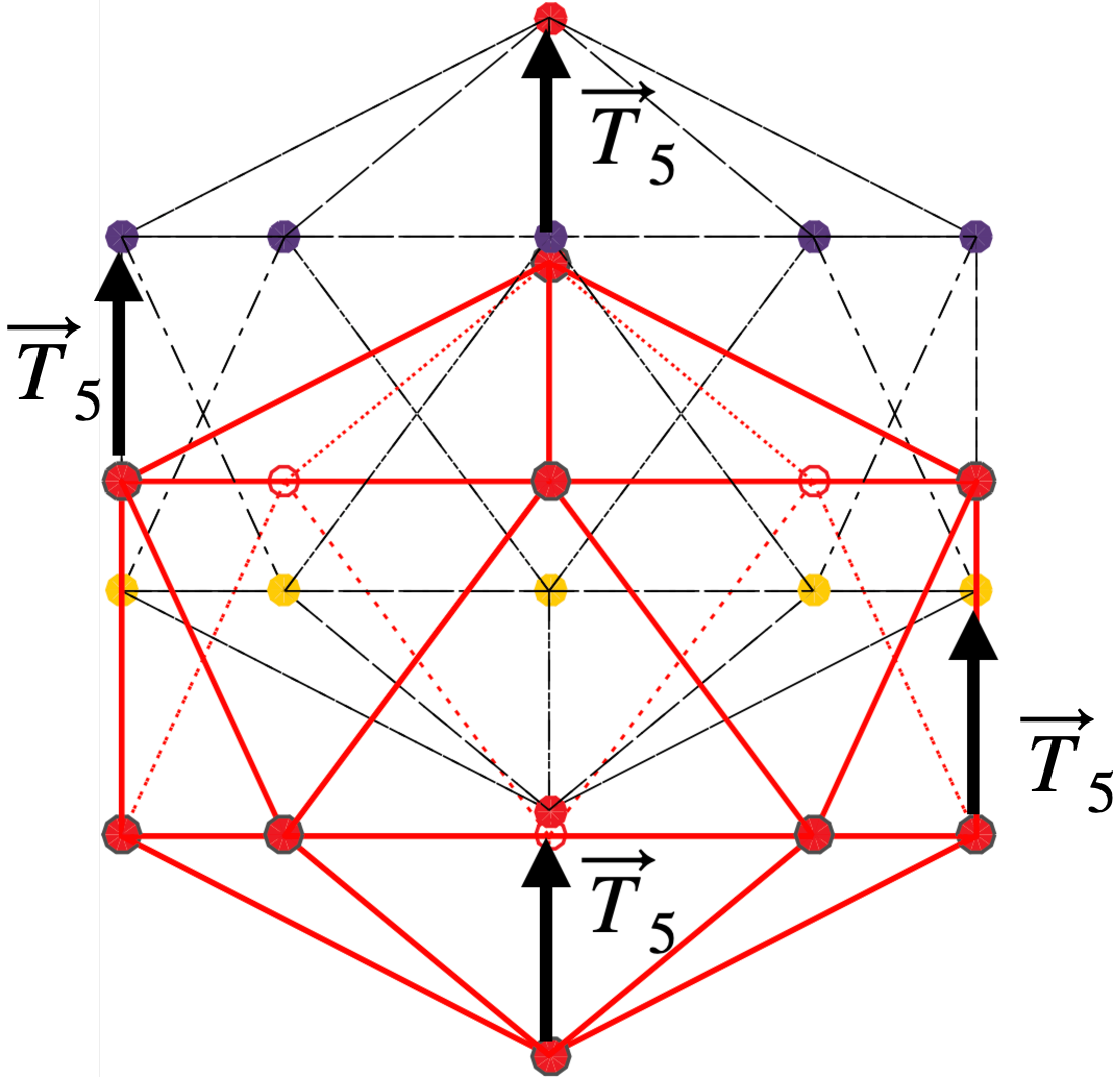
\includegraphics[width=\textwidth]{images/p_arr_construction_2.pdf}
		\caption{Shift icosahedron by a translation vector. Mathematically this is \mbox{\(\mathcal{I}\vec{v} \cup (\mathcal{I}\vec{v} + \vec{t})\)}.}
	\end{subfigure}
	\hfill
	\begin{subfigure}{0.35\textwidth}
		\centering
		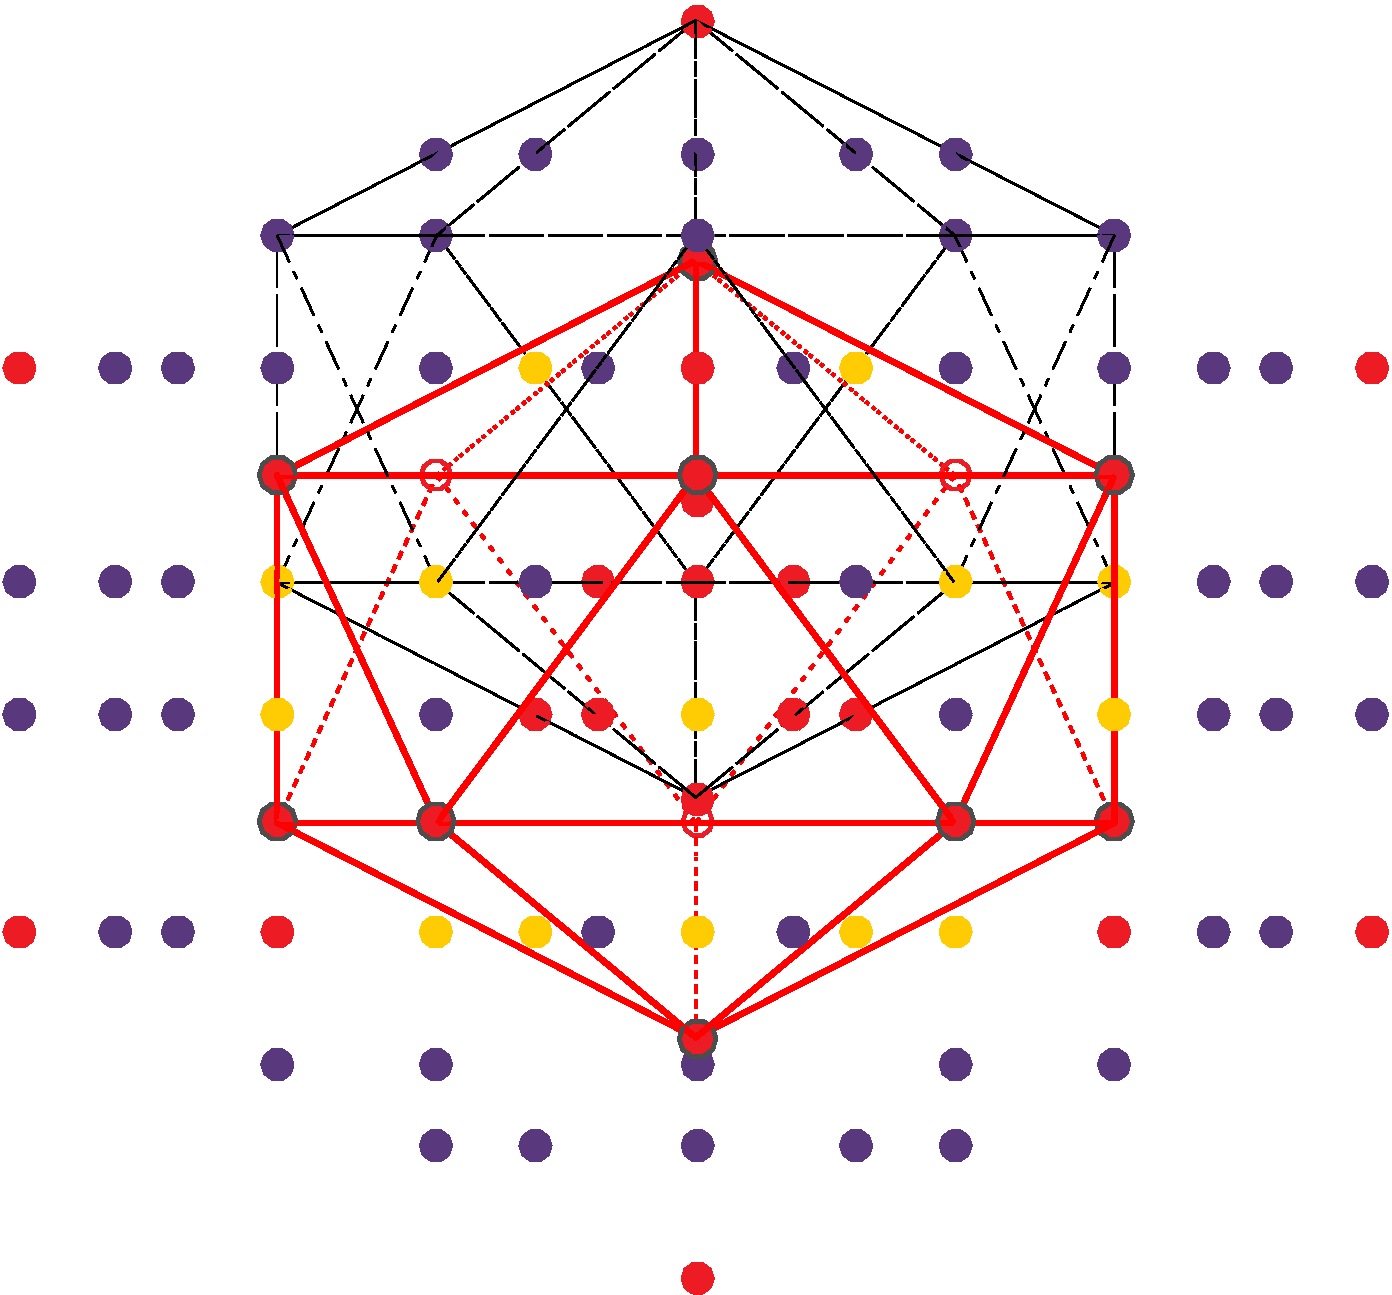
\includegraphics[width=\textwidth]{images/p_arr_construction_3.pdf}
		\caption{Reapply icosahedral symmetry, getting the final expression \(\mathcal{I}\vec{v} \cup (\mathcal{I}\vec{v} + \mathcal{I}\vec{t})\).}
	\end{subfigure}
	\caption{The process of creating a one-base point array. Graphics from Dr. Dave Wilson.}
	\label{fig:point_array_construction}
\end{figure}

\section{Transitions Between Point Arrays}
\subsection{Viral Maturation}
\todo[inline]{Give a less mathy description of the virus transition problem \\ describe goals about preserving symmetry}

\section{Mathematical View of the Problem}
Our desire to find transitions between point arrays that preserving some or all of icosahedral symmetry.
In order to find such transitions, we need to understand this problem mathematically.
On the highest level of abstraction, we are simply solving matrix equations of the form \[TB_0 = B_1.\]
In this equation, \(B_0\) and \(B_1\) represent the native and mature point arrays respectively, and \(T\) is our desired linear transformation that preserves icosahedral symmetry.
\footnote{Recall that we realize icosahedral symmetry as a matrix group and icosahedral point arrays are sets of vectors, so it makes sense that we are solving a matrix equation.}
Because we want to represent the point arrays, there is a specific structure to the \( B_0 \) and \( B_1 \) matrices.
Let us call us these matrices \emph{point array matrices}.
Before we define a point array matrix, we introduce a new notation called \emph{bar notation}.
\newcommand{\icobar}[1]{\overline{\vec{#1}}}

\begin{Definition}[Icosahedral Bar Notation]
	%\newcommand{\icobar}[2]{\overline{\vec{#1}_{#2}}}
	Let \(\vec{v}\) be a 6-dimensional vector.
	Then we define that \(\icobar{v}\) is an element of the icosahedral orbit of \(\vec{v}\).
	That is, \(\icobar{v} \in \mathcal{I}\vec{v}\).
	
	\todo[inline]{perhaps I change it to this notation: \( \overset{\mathcal{I}}{\overline{\vec{v}}} \) ?\\ ask Dr. Oloo about this...}
\end{Definition}
This definition allows us to easily denote when we wish to represent an element of the icosahedral orbit of a vector.
With this notation in hand, we can now define a point array matrix.
\begin{Definition}[Point Array Matrix]
	Let \(P\) be a given point array.
	\( P \) is generated by vectors \(\vec{t}, \vec{v}_1, \vec{v}_2, \dots, \vec{v}_n\).
	\todo[color=red]{fix the bold face in subscript of \texttt{icobar} command}
	A \emph{point array matrix} is a \( 6 \times (n+1) \) matrix of the form \[\begin{bmatrix}
		| & | & | & \cdots & | \\
		\icobar{t} & \icobar{v_1} & \icobar{v_2} & \cdots & \icobar{v_n} \\
		| & | & | & \cdots & | 
	\end{bmatrix}\]
	whose rank is either equal to the minimum of \( n+1 \) and 6.
	Notice that because we are using the icosahedral bar notation defined earlier, this definition is representing a class of matrices that all correspond to the same point array.
	That is, we are defining the form of any representative of the given point array \( P \).
	Denote the set of point array matrices for \( P \) as \( \pam(P) \).
\end{Definition}
The \( B_0 \) and \( B_1 \) matrices are both point array matrices and so both have this general form for their respective point arrays.

One fact that will be useful to know is how many point array matrices there are for a singular point array.
Let \( P \) be a point array.
If we let \( m \) be the number of point array matrices for \( P \) then
\[m \leq \abs{\mathcal{I}\vec{t}} \cdot \abs{\mathcal{I}\vec{v}_1} \cdot \abs{\mathcal{I}\vec{v}_2} \cdot \dots \cdot \abs{\mathcal{I}\vec{v}_n}.\]
We can only say for certain that \( m \) is less than or equal to this value because we require point array matrices to be linearly independent (or have rank 6).
\footnote{If we have that \( \vec{v}_i = \vec{v}_j \) with \( i \neq j \), then there are matrices of the correct form that are not linearly independent.}
However, in general we can assume that \( m \) is equal to this value since in general all the generating vectors are distinct.

\subsection{Mathematically Describing Transitions}
We have defined what the \( B_0 \) and \( B_1 \) matrices look like, now we define the nature of the \( T \) matrix.
A transition \(T\) that preserves all of icosahedral symmetry must have the form: \begin{equation} \label{eq:ico-transition}
	T = \begin{bmatrix}
		z  & x  & -x & -x & x  & x \\
		x  & z  & x  & -x & -x & x \\
		-x & x  & z  & x  & -x & x \\
		-x & -x & x  & z  & x  & x \\
		x  & -x & -x & x  & z  & x \\
		x  & x  & x  & x  & x  & z
\end{bmatrix}\end{equation}

Our linear transformation \(T\) preserves icosahedral symmetry because it is in the centralizer of \(\mathcal{I}\) (or one its of maximal subgroups).
\begin{Definition}[Centralizer]
	The centralizer of a group \(G\), denoted by \(Z(G)\) is the set of elements that commute with all elements of \(G\).
	That is, \[Z(G) = \{z\ |\ gz = zg\ \forall g \in G\}.\]
\end{Definition}
Any matrix of the form given in equation \ref{eq:ico-transition} is in \(Z(\mathcal{I})\), the centralizer of \(\mathcal{I}\).
Below are the general matrix forms for \(Z(A_4)\), \(Z(D_{10})\), and \(Z(D_6)\). \cite{indelicatoetal2012}
\begin{align}
	\begin{bmatrix}
		z  & -x & -y & -t & t  & -x \\
		t  & z  & t  & x  & x  & y  \\
		-y & -x & z  & t  & -t & -x \\
		x  & -t & -x & z  & y  & t  \\
		-x & -t & x  & y  & z  & t  \\
		t  & y  & t  & -x & -x & z
	\end{bmatrix} \in Z(A_4) \\
	\begin{bmatrix}
		z & x & y & y & x & t \\
		x & z & x & y & y & t \\
		y & x & z & x & y & t \\
		y & y & x & z & x & t \\
		x & y & y & x & z & t \\
		u & u & u & u & u & w
	\end{bmatrix} \in Z(D_{10}) \\
	\begin{bmatrix}
		u  & w  & -w & x  & s  & s  \\
		-t & y  & v  & -v & z  & -t \\
		t  & v  & y  & v  & t  & -z \\
		z  & -v & v  & y  & -t & -t \\
		s  & x  & -w & w  & u  & s  \\
		s  & w  & -x & w  & s  & u
	\end{bmatrix} \in Z(D_{6})
\end{align}

\subsection{Transitions Preserving Symmetry}
\todo[inline]{Talk about why we want the centralizer here}

% order of these two sections?
\subsection{How To Find Transitions}
We now understand the mathematical structures of this problem.
The question now is what procedure should we use in order to find transitions that preserve symmetry.

Suppose we want to a symmetry preserving transition from point array \( P \) to point array \( Q \).
Then to find this transition, we need to find a point array matrix \( B_0 \in \pam(P) \) and a point array matrix \( B_1 \in \pam(Q) \) such that the equation \( TB_0 = B_1 \) can be solved for \( T \).
Thus we if wish to find a transition preserving icosahedral symmetry, then our equation looks like
\begin{equation}
	\begin{bmatrix}
		z  & x  & -x & -x & x  & x \\
		x  & z  & x  & -x & -x & x \\
		-x & x  & z  & x  & -x & x \\
		-x & -x & x  & z  & x  & x \\
		x  & -x & -x & x  & z  & x \\
		x  & x  & x  & x  & x  & z
	\end{bmatrix}
	\cdot
	\begin{bmatrix}
		| & | & | & \cdots & | \\
		\icobar{t} & \icobar{v_1} & \icobar{v_2} & \cdots & \icobar{v_n} \\
		| & | & | & \cdots & |
	\end{bmatrix}
	=
	\begin{bmatrix}
		| & | & | & \cdots & | \\
		\icobar{t'} & \icobar{u_1} & \icobar{u_2} & \cdots & \icobar{u_n} \\
		| & | & | & \cdots & |
	\end{bmatrix}
	\label{eq:general-ico-equation}
\end{equation}
where \( P \) is generated by vectors \(\vec{t}, \vec{v}_1, \vec{v}_2, \dots, \vec{v}_n\) and \( Q \) is generated by vectors \(\vec{t}, \vec{u}_1, \vec{u}_2, \dots, \vec{u}_n\).
\footnote{
	Is it possible that \( P \) and \( Q \) are generated by an unequal number vectors which would cause this equation to be invalid. 
	There is a way to make the equation work when this is case and will be described later.
	}
Because \( \pam(P) \) and \( \pam(Q) \) are sets of matrices, equation \ref{eq:general-ico-equation} describes a set of equations, whose cardinality is equal to \( \abs{\pam(P)}\cdot\abs{\pam(Q)}\).
Therefore, to find an icosahedral symmetry preserving transition, we must find an equation within this set that is solvable.
\footnote{
	One may notice that by how this equation is setup, the order of the generators matters.
	This is in constrast to the definition of an icosahedral point array, where the order doesn't matter.
	In truth, the permutation of the columns of both \( B_0 \) and \( B_1 \) doesn't matter (except for the first columns, which must remain first) and so the true number of equations is multiplied by \( n!^2 \).
	Thus the true number of equations that must be checked for the transition \( P \to Q \) is \( n!^2\cdot\abs{\pam(P)}\cdot\abs{\pam(Q)} \).
	However, when I actually compute these transitions, I consider the various permutations of the generators as separate cases entirely and thus can forgo talking about permutations when finding transitions.
	}

\subsection{CCMV \( D_6 \) Transition Example}


\section{Computational Techniques}
\todo[inline]{
	Describe the nature of this problem computationally \\ 
	- Embarassingly parallel \\
	- How to store this data \\
	- More...?
}

\todo[inline]{Talk about how we can build up \( B0 \) and \( B1 \) matrices one vector at a time}

\subsection{C++ Program}
\subsubsection{Entry Sampling}
\subsubsection{Partial Transitions}
\subsubsection{Contrapositive}
\todo[inline]{- Norm checking\\
- Checking mapping into the ending point array
}

\subsubsection{Parallelization}

\subsection{Python Program}
\subsubsection{Pair Checking}
\todo[inline]{this will involve the subsets of \( \mathcal{I} \times \mathcal{I} \) idea}
\subsubsection{Depth first search}
\todo[inline]{this is the current version running on Jigwe}
\subsubsection{Parallelization}

\section{Results}
After doing these computational methods, I found intriguing results, summarized by the following:
\begin{enumerate}
	\item These methods produce the same four \( D_6 \) transition matrices for CCMV given in \cite{indelicatoetal2012}.
	
	\item These methods allow us to find all symmetry preserving transitions exist between all of the 55 standard one-base point arrays. Larger point arrays must be built from these 55, so this data also helps in determining what transitions are and are not possible between bigger point arrays.
	
	\item There cannot exist any transition that preserves all of icosahedral symmetry between any different point arrays, since no such icosahedral symmetry preserving transition exists between any of the 55 standard point arrays.
		We can only find transitions that preserve the maximal subgroups \(D_6, D_{10}, \text{ and } A_4\).
	
	\item \todo[inline]{Talk about 2+ base results; comprehensive 2 base running on Jigwe currently}
\end{enumerate}

\section{Acknowledgements}
\begin{itemize}
	\item Heyl Scholarship Research Fund
	\item Dr. Stephen Oloo and Dr. Dave Wilson
	\item Dr. Dave Wilson and Dr. Sandino Vargas-Perez for allowing me to use the Kalamazoo College supercomputer Jigwe.
\end{itemize}


\medskip
\bibliographystyle{unsrt}%Used BibTeX style is unsrt
\bibliography{references}

\end{document}
